\section{Reproducibility: systems, data, architecture, and training}
\label{app:repro}

This appendix records the systems, data-generating distributions, network architectures, and training
protocol used in Section~\ref{sec:experiments}. The SIR and Lotka--Volterra models are given in full
below; the OGTT ISS model has a large secretion/incretin subsystem that we do not reproduce in its
entirety here, deferring its full equations and fixed physiological constants to the source
implementation~\cite{ha2024iss} and the released code. Exact reproduction of every reported number
therefore requires the accompanying code at the fixed commit (Appendix~\ref{app:repro-code}); the values
below are taken from that configuration.

\subsection{Benchmark systems and governing equations}
\label{app:repro-systems}

Each system is integrated as an initial value problem with \texttt{scipy.integrate.solve\_ivp} at the
listed sampling times; a single state variable is observed and the rest is treated as hidden. Parameters
are treated as constant augmented states for the observability analysis of Section~\ref{sec:identifiability}.

\paragraph{SIR (epidemiological)} With $N=S+I+R$ conserved,
\[
\dot S=-\frac{\beta S I}{N},\qquad
\dot I=\frac{\beta S I}{N}-\gamma I,\qquad
\dot R=\gamma I,
\]
observed variable $S$, hidden variable $I$, parameters $\theta=(\beta,\gamma)$. Fixed initial condition
$(S_0,I_0,R_0)=(49,1,0)$. Priors: $\beta,\gamma$ uniform, on the \emph{wide} range
$\beta,\gamma\sim\mathcal{U}[0.01,0.5]$ (a \emph{narrow} variant uses $\beta\sim\mathcal{U}[0.08,0.12]$,
$\gamma\sim\mathcal{U}[0.09,0.11]$). The ODE is integrated on $[0,110]$ and observations are taken on the
uniform grid $t=\mathrm{linspace}(0,100,N_\mathrm{obs})$ with $N_\mathrm{obs}$ points ($N_\mathrm{obs}=8$ for
the main runs; the density sweep uses $N_\mathrm{obs}\in\{4,8,16,30\}$); the extra interval past the last
observation is a small integration buffer.

\paragraph{Lotka--Volterra (ecological)}
\[
\dot x=\alpha x-\beta x y,\qquad
\dot y=\delta x y-\gamma y,
\]
observed prey $x$, hidden predator $y$, parameters $\theta=(\alpha,\beta,\delta,\gamma)$. Priors
$\alpha\sim\mathcal{U}[0.6,1.0]$, $\beta\sim\mathcal{U}[0.4,0.8]$, $\delta\sim\mathcal{U}[0.2,0.6]$,
$\gamma\sim\mathcal{U}[0.6,1.0]$; initial conditions $x_0\in[5,15]$, $y_0\in[1,5]$ accepted by
rejection so that the conserved-energy offset $\Delta V=V(x_0,y_0)-V(x_{\mathrm{eq}},y_{\mathrm{eq}})$ lies
in $[0.1,1.5]$ (ensuring non-trivial oscillations), where $V(x,y)=\delta x-\gamma\log x+\beta y-\alpha\log y$
is the standard Lotka--Volterra conserved quantity and $(x_{\mathrm{eq}},y_{\mathrm{eq}})=(\gamma/\delta,\alpha/\beta)$.
Time span $[0,20]$, $10$ uniform samples $t=\mathrm{linspace}(0,20,10)$.

\paragraph{OGTT (physiological, full ISS model)} The glucose equation is~\eqref{eq:ogtt-glucose}, coupled
to insulin and a two-stage incretin delay chain,
\[
\dot I=\frac{b\,\mathrm{ISR}(N_5;S_I,\sigma)}{\mathrm{BV}}-k\,I,\qquad
\dot N_5,\ \dot N_6:\ \text{incretin delay dynamics},
\]
with hepatic glucose production $\mathrm{HGP}(S_I,I)$ as in Section~\ref{subsec:exp-ogtt}. Observed glucose
$G$, hidden insulin $I$, parameters $\theta=(S_I,\sigma)$. Parameters and the initial glucose/insulin are
drawn from data-driven log-normal priors (\texttt{scipy.stats.lognorm}, rejection-sampled for strict
positivity), and $(N_{5,0},N_{6,0})$ are set to the algebraic steady state given $G_0$:
writing $\mathrm{LogN}(s,\mathrm{loc},\mathrm{scale})$ for the \texttt{scipy.stats.lognorm} parameters,
\[
S_I\sim\mathrm{LogN}(0.527,-0.105,0.506),\quad
\sigma\sim\mathrm{LogN}(0.593,-0.053,0.543),
\]
\[
G_0\sim\mathrm{LogN}(0.286,60.07,29.81),\quad
I_0\sim\mathrm{LogN}(0.596,-0.013,6.495).
\]
Time span $[0,120]$; the sparse clinical $30$-minute grid $t\in\{0,30,60,90,120\}$ ($5$ points). The fixed
physiological constants ($E_{G0}$, $b$, $k$, $\mathrm{BV}$, the HGP and incretin coefficients) are those of
the released ISS implementation~\cite{ha2024iss}.

\paragraph{Observations} All training/test data in Section~\ref{sec:experiments} are \emph{noiseless}
deterministic ODE integrations (the stochastic-forcing option and the derivative-feature option are
disabled). The difficulty comes from the ambiguity and ill-conditioning induced by partial, sparse
sampling --- not from added measurement noise; SIR is an identifiable control, whereas Lotka--Volterra and
the full OGTT model are, respectively, unidentifiable and only weakly/locally identifiable from partial
observations.

\subsection{Data splits and normalization}
\label{app:repro-norm}

Sample sizes: OGTT $5\times10^4$, SIR $2.6\times10^4$, Lotka--Volterra $2\times10^4$ trajectories. Each set
is partitioned $60/20/20$ into train/validation/test with a fixed seed, the split performed \emph{before}
normalization so that the normalizer is fit on the training set only (no leakage). For the SIR
generalization discussion we additionally use a parameter-\emph{extrapolation} (out-of-distribution) test
split; unless noted, results use the standard random split.

Normalization: observed and hidden states are divided by a per-variable scale (the training-set maximum
absolute value). Parameters are mapped to $[-1,1]$ by a min--max transform fit on the training set with a
$10\%$ margin; for OGTT this is applied after a $\log$ transform (so the multiplicative $S_I\sigma$
structure becomes additive), while SIR and LV use the plain min--max. Denormalization inverts these maps.
The fixed-point iteration is initialized at $\theta^{(0)}$, the geometric mean of the training parameters.

\subsection{Network architecture and matched-branch direct baseline}
\label{app:repro-arch}

Both $H_\phi$ and $P_\psi$ are multilayer perceptrons with hidden widths $[256,256,256]$ and SiLU
activations. When spectral normalization is enabled, every linear layer is spectrally normalized
(one power iteration) and each hidden block is rescaled by a fixed per-layer factor $0.9$
(the \texttt{ExcludeLambda} module); $P_\psi$ additionally ends in a $\tanh$, which bounds its output to
the normalized box $[-1,1]^p$ and thereby guarantees $\mathcal{T}(\cdot;\mathbf{x}_\mathrm{obs})$ maps
$\Theta$ into $\Theta$ (Section~\ref{subsec:exp-convergence}). Weights use orthogonal initialization.
Parameter counts (spectral-normalized): for OGTT, $|\phi|=134{,}917$ and $|\psi|=134{,}914$
($\approx2.70\times10^5$ total); SIR $\approx2.69\times10^5$; Lotka--Volterra $\approx2.76\times10^5$.

The \emph{matched-branch direct baseline} (\texttt{SingleNetworkBaseline}) maps $\mathbf{x}_\mathrm{obs}
\mapsto\theta$ through the \emph{same} MLP backbone --- identical hidden widths $[256,256,256]$, SiLU
activations, spectral normalization, initialization, optimizer, and data split --- as a single network
($\approx1.33$--$1.35\times10^5$ parameters, i.e.\ one branch of the operator). This baseline therefore has
the \emph{same per-network hidden widths} as each branch of the operator, but is \emph{not} matched in total
parameter count: the decoupled operator uses two such networks ($H_\phi$ and $P_\psi$) and hence roughly twice
the parameters. The comparison thus isolates the effect of the decoupled reconstruction structure at equal
per-network width, and if anything gives the operator a capacity advantage rather than a handicap. One
architectural asymmetry matters downstream: $P_\psi$ ends in a $\tanh$ that bounds the operator's parameter
output to $\Theta$, whereas the direct baseline has an unbounded linear output head.

\subsection{Training and inference hyperparameters}
\label{app:repro-train}

\begin{table}[h]
\centering
\caption{Training and inference configuration (identical across the three systems unless a value is
listed per system).}
\label{tab:hyperparams}
{\small
\begin{tabular}{ll}
\hline
Setting & Value \\
\hline
Optimizer & Adam, learning rate $10^{-3}$, weight decay $0$ \\
LR schedule & \texttt{ReduceLROnPlateau} (factor $0.9$, patience $200$, min $10^{-8}$) \\
Batch size & $256$ \\
Epochs (max) & $1000$ (SIR, LV); $1500$ (OGTT) \\
Early stopping & on validation loss, patience $150$ (SIR, LV) / $250$ (OGTT), min-delta $10^{-6}$ \\
Training losses & decoupled teacher forcing: $\mathcal{L}_H+\mathcal{L}_P$ (both MSE), Eqs.~\eqref{eq:loss_h}--\eqref{eq:loss_p} \\
Spectral-norm scale & $0.9$ per hidden layer (contraction runs) \\
Inference iterations & $K=10$ fixed-point steps from $\theta^{(0)}$ \\
Random seed & $42$ (data generation, split, and torch) \\
\hline
\end{tabular}
}
\end{table}

The main recovery numbers (Table~\ref{tab:recovery}) and the trained-operator figures come from single-seed
runs (seed $42$) of the full training pipeline; retraining that pipeline across many seeds for all three
systems is GPU-bound and, due to computational constraints, was not carried out here, so we report
point values there. Where multi-seed evidence is inexpensive we do provide it: the coordinate-MSE ablation
of Section~\ref{subsec:exp-ogtt} is run over five seeds and reported as mean\,$\pm$\,std, and it confirms
that the qualitative conclusions (the on/off-fiber behavior and the individual-coordinate recovery) are
seed-stable. The certified contraction constant and the test-set-wide residual/error statistics of
Section~\ref{subsec:exp-convergence} are computed from the saved checkpoint of the main OGTT run.

\subsection{Test-time perturbation stress test}
\label{app:repro-noise}

This appendix collects the full sweep behind Section~\ref{subsec:exp-noise}. The protocol is fixed before
evaluation: independent additive Gaussian noise $x'_{ij}=x_{ij}+\alpha s_j\epsilon_{ij}$ on each observed
channel, $s_j$ the clean training-set channel standard deviation, $\alpha\in\{0,0.005,0.01,0.02,0.05,0.10\}$,
injected in physical units and re-normalized with the clean-training map; $30$ noise replicates per clean
test trajectory; the identical perturbed observations fed to all three estimators; a single training seed
($42$), since retraining is compute-bound. The failure rate counts a prediction as failed if any coordinate
is non-finite, non-positive, or outside the training-parameter support $[\min,\max]$; success-conditioned
errors are always reported with the failure rate, and no failed sample is dropped from the counts. Metrics
use per-point quantities: the per-point product $S_I\sigma$ and its signed/absolute error (a per-bin mean of
on-fiber predictions would itself be off-fiber by Jensen, so we avoid it).

\begin{figure}[h]
\centering
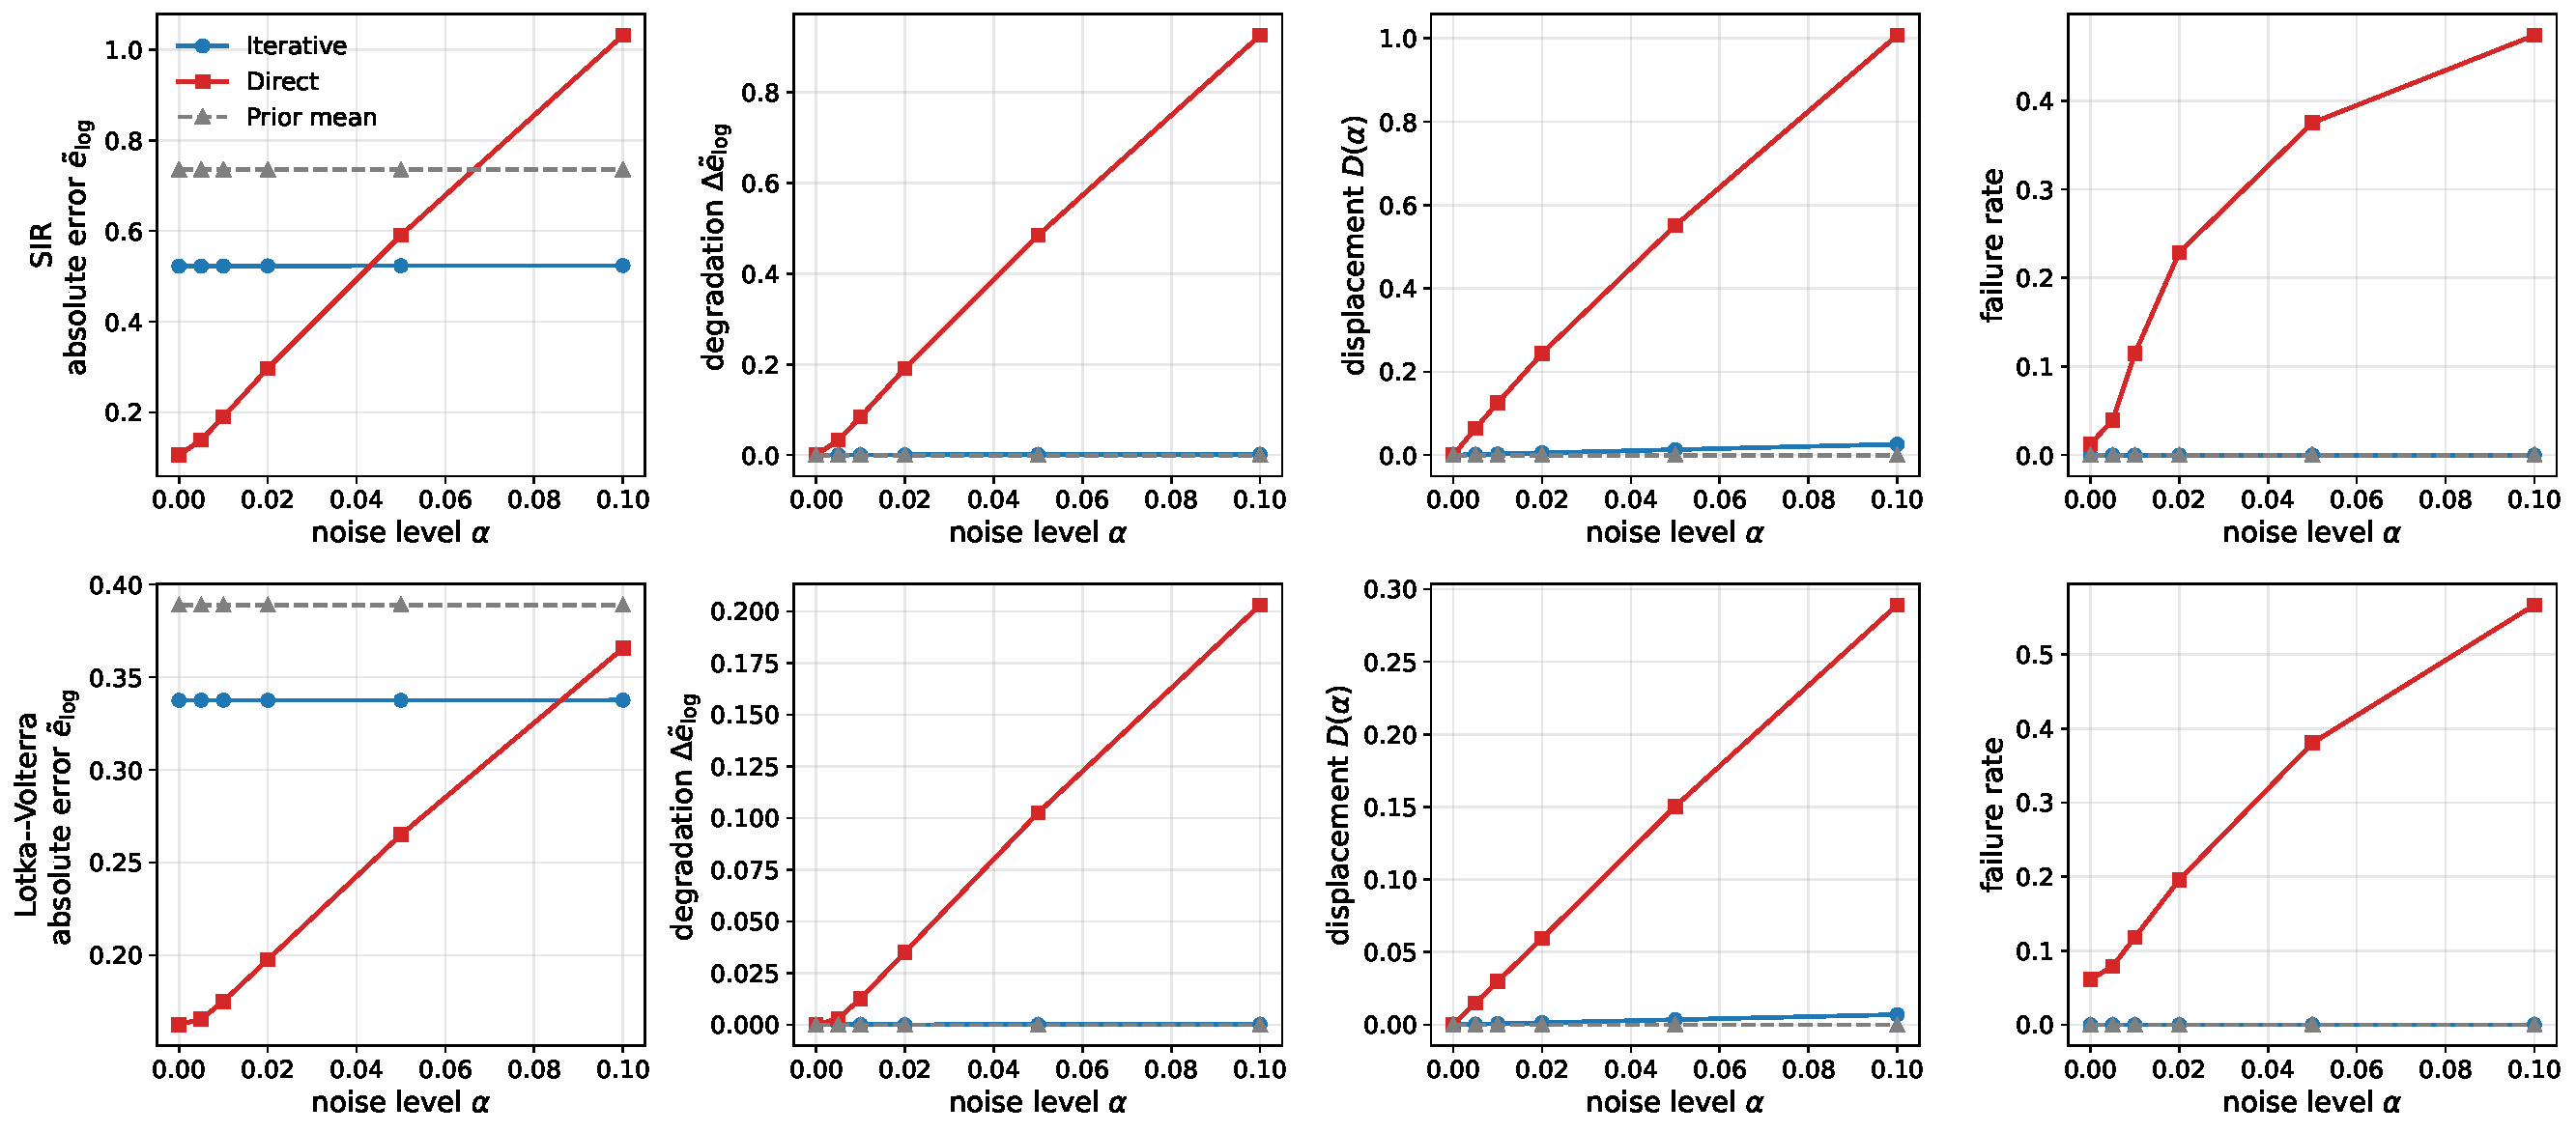
\includegraphics[width=\textwidth]{figures/exp/noise_sir_lv_2x2.pdf}
\caption{Test-time noise response for SIR (top) and Lotka--Volterra (bottom): absolute error, degradation,
displacement, and failure rate versus $\alpha$. The same ordering as OGTT (Figure~\ref{fig:noise-ogtt})
holds: the direct regressor is most accurate when clean but degrades and violates support under noise, the
iterative operator is flat at a higher floor, and the prior mean is flat and inaccurate. For LV the direct
regressor already fails on $6\%$ of clean test samples --- a reflection of the exact prey-only ambiguity of
Section~\ref{subsec:exp-lv}, which places part of the fiber outside the training support even before noise.}
\label{fig:noise-sir-lv}
\end{figure}

\paragraph{Bias/variance decomposition.} For each clean test trajectory we average the log-coordinate
prediction over the $30$ replicates, $\bar z_i=\tfrac1R\sum_r\log\hat\theta(x_i^{(r)})$, and split the
error into $\mathrm{bias}^2_i=\|\bar z_i-\log\theta_i\|^2$ and noise variance
$\tfrac1R\sum_r\|\log\hat\theta(x_i^{(r)})-\bar z_i\|^2$ (finite subset). At $\alpha=0.10$ the iterative
operator is almost pure bias (SIR/OGTT/LV squared bias $0.94/0.54/0.13$, noise variance
$1.3{\times}10^{-3}/1.0{\times}10^{-3}/1.4{\times}10^{-4}$), whereas the direct regressor's variance
dominates ($2.1/29/0.23$) on a smaller bias ($0.24/1.2/0.05$). The flat degradation curve of the iterative
estimator is therefore a low-variance, high-bias signature, not preserved information. The raw per-replicate
aggregates are saved as \path{results/det_meanlocus/noise_stress_test.csv}.

\paragraph{Scope.} We ran only the pre-registered primary family (independent additive observation noise).
Secondary families (trajectory-level calibration shift, sampling-time jitter, quantization, and
singular-direction perturbations) are deliberately left to future work; the primary sweep already answers
the stated question --- how the two point estimators trade clean accuracy against perturbation sensitivity ---
and we stop rather than expand the noise model until an ordering emerges.

\subsection{Code and scripts}
\label{app:repro-code}

% TODO(authors): once the repository is public, replace the sentence below with:
%   ``The code, configurations, and analysis scripts are available at \url{<URL>} (commit <hash>).''
The code, configurations, and analysis scripts will be released publicly upon publication, at a fixed
commit that reproduces every reported number. The experiments of this pass are reproduced by standalone
scripts under \path{experiments/det_meanlocus/}:
\path{condmean_locus_fig.py} (conditional-mean locus, Figure~\ref{fig:ogtt-condmean}),
\path{ogtt_observability.py} (full- vs constant-HGP sampled sensitivity, Figure~\ref{fig:ogtt_hgp}),
\path{certify_contraction.py} (contraction certification),
\path{coord_mse_ablation.py} (physical- vs log-coordinate MSE ablation, Figure~\ref{fig:ogtt-coord}), and
\path{noise_stress_test.py} together with \path{noise_report.py} (the test-time perturbation sweep,
Table~\ref{tab:noise} and Figures~\ref{fig:noise-ogtt}--\ref{fig:noise-sir-lv}).
Model training uses \path{run_paper_exp.py} with the settings of Table~\ref{tab:hyperparams}.
